% ------------------------------------------------------------------------
% ------------------------------------------------------------------------
% abnTeXf2: Modelo de Trabalho Academico (tese de doutorado, dissertacao de
% mestrado e trabalhos monograficos em geral) em conformidade com 
% ABNT NBR 14724:2011: Informacao e documentacao - Trabalhos academicos -
% Apresentacao
% ------------------------------------------------------------------------
% ------------------------------------------------------------------------

\documentclass[
	% -- opções da classe memoir --
	12pt,				% tamanho da fonte
	openright,			% capítulos começam em pág ímpar (insere página vazia caso preciso)
	oneside,			% para impressão em verso e anverso. Oposto a oneside
	a4paper,			% tamanho do papel. 
	% -- opções da classe abntex2 --
	%chapter=TITLE,		% títulos de capítulos convertidos em letras maiúsculas
	%section=TITLE,		% títulos de seções convertidos em letras maiúsculas
	%subsection=TITLE,	% títulos de subseções convertidos em letras maiúsculas
	%subsubsection=TITLE,% títulos de subsubseções convertidos em letras maiúsculas
	% -- opções do pacote babel --
	english,			% idioma adicional para hifenização
	french,				% idioma adicional para hifenização
	spanish,			% idioma adicional para hifenização
	brazil,				% o último idioma é o principal do documento
	oldfontcommands
	]{abntex2}

% ---
% Pacotes básicos 
% ---
\usepackage{lmodern}			% Usa a fonte Latin Modern			
\usepackage[T1]{fontenc}		% Selecao de codigos de fonte.
\usepackage[utf8]{inputenc}		% Codificacao do documento (conversão automática dos acentos)
\usepackage{lastpage}			% Usado pela Ficha catalográfica
\usepackage{indentfirst}		% Indenta o primeiro parágrafo de cada seção.
\usepackage{color}				% Controle das cores
\usepackage{graphicx}			% Inclusão de gráficos
\usepackage{microtype} 			% para melhorias de justificação
\usepackage{eurosym}			% habilita símbolo do Euro
% ---
		
% ---
% Pacotes adicionais, usados apenas no âmbito do Modelo Canônico do abnteX2
% ---
\usepackage{lipsum}				% para geração de dummy text
% ---

% ---
% Pacotes de citações
% ---
\usepackage[brazilian,hyperpageref]{backref}	 % Paginas com as citações na bibl
\usepackage[num]{abntex2cite}	% Citações padrão ABNT


% --- 
% CONFIGURAÇÕES DE PACOTES
% --- 

% ---
% Configurações do pacote backref
% Usado sem a opção hyperpageref de backref
\renewcommand{\backrefpagesname}{Citado na(s) página(s):~}
% Texto padrão antes do número das páginas
\renewcommand{\backref}{}
% Define os textos da citação
\renewcommand*{\backrefalt}[4]{
	\ifcase #1 %
		Nenhuma citação no texto.%
	\or
		Citado na página #2.%
	\else
		Citado #1 vezes nas páginas #2.%
	\fi}%
% ---

% ---
% Informações de dados para CAPA e FOLHA DE ROSTO
% ---
\titulo{SISTEMA DE GERENCIAMENTO DE ENERGIA PARA CUBESAT}
\autor{ARNALDO ALVES VIANA JÚNIOR\\
OTÁVIO MOREIRA PETITO\\
TIAGO AUGUSTO ORCAJO DEMAY CORDEIRO}
\local{SÃO CAETANO DO SUL}
\data{2015}
\orientador{Prof. Me. Alessandro de Oliveira Santos}
%\coorientador{Professor}
\instituicao{Escola de Engenharia Mauá}
%tipotrabalho{Tese (Trabalho de Conclusão de Curso)}
% O preambulo deve conter o tipo do trabalho, o objetivo, 
% o nome da instituição e a área de concentração 
\preambulo{Trabalho de Conclusão de Curso apresentado à Escola de Engenharia Mauá do Centro Universitário do Instituto Mauá de Tecnologia, como parte dos requisitos necessários à obtenção do grau de bacharel em Engenharia na habilitação Engenharia Eletrônica. Área de concentração: Engenharia Elétrica}
% ---


% ---
% Configurações de aparência do PDF final

% alterando o aspecto da cor azul
\definecolor{blue}{RGB}{41,5,195}

% informações do PDF
\makeatletter
\hypersetup{
     	%pagebackref=true,
		pdftitle={\@title}, 
		pdfauthor={\@author},
    	pdfsubject={\imprimirpreambulo},
	    pdfcreator={LaTeX with abnTeX2},
		pdfkeywords={abnt}{latex}{abntex}{abntex2}{trabalho acadêmico}, 
		colorlinks=true,       		% false: boxed links; true: colored links
    	linkcolor=black,          	% color of internal links
    	citecolor=black,        		% color of links to bibliography
    	filecolor=black,      		% color of file links
		urlcolor=black,
		bookmarksdepth=4 
}
\makeatother
% --- 

% --- 
% Espaçamentos entre linhas e parágrafos 
% --- 

% O tamanho do parágrafo é dado por:
\setlength{\parindent}{1.25cm}

% Controle do espaçamento entre um parágrafo e outro:
\setlength{\parskip}{0.2cm}  % tente também \onelineskip

% ---
% compila o indice
% ---
\makeindex
% ---

% ----
% Início do documento
% ----
\begin{document}

% Retira espaço extra obsoleto entre as frases.
\frenchspacing 
% ----------------------------------------------------------
% ELEMENTOS PRÉ-TEXTUAIS
% ----------------------------------------------------------
% \pretextual

% ---
% Capa
% ---
\imprimircapa
% ---

% ---
% Folha de rosto
% (o * indica que haverá a ficha bibliográfica)
% ---
\imprimirfolhaderosto*
% ---

% ---
% Inserir a ficha bibliografica
% ---

% Isto é um exemplo de Ficha Catalográfica, ou ``Dados internacionais de
% catalogação-na-publicação''. Você pode utilizar este modelo como referência. 
% Porém, provavelmente a biblioteca da sua universidade lhe fornecerá um PDF
% com a ficha catalográfica definitiva após a defesa do trabalho. Quando estiver
% com o documento, salve-o como PDF no diretório do seu projeto e substitua todo
% o conteúdo de implementação deste arquivo pelo comando abaixo:
%
% \begin{fichacatalografica}
%     \includepdf{fig_ficha_catalografica.pdf}
% \end{fichacatalografica}
\begin{fichacatalografica}
	\vspace*{\fill}					% Posição vertical
	\hrule							% Linha horizontal
	\begin{center}					% Minipage Centralizado
	\begin{minipage}[c]{12.5cm}		% Largura
	
	Júnior, Arnaldo Alves Viana
	
	\hspace{0.5cm} \imprimirtitulo  / Arnaldo Alves Viana Júnior, Otávio Moreira Petito e Tiago Augusto Orcajo Demay. --
	\imprimirlocal, CEUN-EEM, \imprimirdata
	
	\hspace{0.5cm} \pageref{LastPage} p. : il. \\
	
	\hspace{0.5cm}
	\parbox[t]{\textwidth}{\imprimirtipotrabalho~--~\imprimirinstituicao,
	\imprimirlocal, \imprimirdata.}\\
	
	\hspace{0.5cm} \imprimirorientadorRotulo~\imprimirorientador\\
	
	\hspace{0.5cm}
		1. Gerenciamento de energia.
		2. CubeSat.
		I. Petito, Otávio Moreira.
		II. Cordeiro, Tiago Augusto Orcajo Demay
		III. Instituto Mauá de Tecnológia. Centro Universitário.
		IV. Sistema de Gerenciamento de Energia para CubeSat\\ 			
	
	\hspace{8.75cm} CDU \\
	
	\end{minipage}
	\end{center}
	\hrule
\end{fichacatalografica}
% ---

% ---
% Inserir errata
% ---

% ---

% ---
% Inserir folha de aprovação
% ---

% Isto é um exemplo de Folha de aprovação, elemento obrigatório da NBR
% 14724/2011 (seção 4.2.1.3). Você pode utilizar este modelo até a aprovação
% do trabalho. Após isso, substitua todo o conteúdo deste arquivo por uma
% imagem da página assinada pela banca com o comando abaixo:
%
% \includepdf{folhadeaprovacao_final.pdf}
%
\begin{folhadeaprovacao}

  \begin{center}
    {\ABNTEXchapterfont\large\imprimirautor}

    \vspace*{\fill}\vspace*{\fill}
    \begin{center}
      \ABNTEXchapterfont\bfseries\Large\imprimirtitulo
    \end{center}
    \vspace*{\fill}
    
    \hspace{.45\textwidth}
    \begin{minipage}{.5\textwidth}
    \end{minipage}%
    \vspace*{\fill}
   \end{center}
        
Trabalho de Conclusão de Curso aprovado em \_\_\_ de \_\_\_\_\_\_\_\_\_\_\_\_\_ de 2015, pela banca examinadora composta por: 

   \assinatura{\textbf{\imprimirorientador} \\ Orientador} 
   \assinatura{\textbf{Professor} \\ Convidado 1}
   \assinatura{\textbf{Professor} \\ Convidado 2}
   %\assinatura{\textbf{Professor} \\ Convidado 3}
   %\assinatura{\textbf{Professor} \\ Convidado 4}
      
   \begin{center}
    \vspace*{0.5cm}
    {\large\imprimirlocal}
    \par
    {\large\imprimirdata}
    \vspace*{1cm}
  \end{center}
  
\end{folhadeaprovacao}
% ---

% ---
% Dedicatória
% ---
% ---

% ---
% Agradecimentos
% ---
\begin{agradecimentos}

A Escola de Engenharia Mauá por fornecer toda a gama de conhecimento e estrutura para um melhor aprendizado.\par
Ao {\imprimirorientador}  pela assessoria prestada quanto ao desenvolvimento do tema.\par
Ao Prof. Rafael Corsi por todo empenho dedicado auxiliando o projeto de distintas maneiras.\par
E aos nossos pais, amigos e namoradas que apesar de todas as dificuldades sempre nos suportaram para o melhor desenvolvimento do projeto.

\end{agradecimentos}
% ---

% ---
% Epígrafe
% ---
\begin{epigrafe}
    \vspace*{\fill}
	\begin{flushright}
		\textit{O maior bem do homem é uma mente inquieta.\\(Isaac Asimov)}
	\end{flushright}
\end{epigrafe}
% ---

% ---
% RESUMOS
% ---

% resumo em português
\setlength{\absparsep}{18pt} % ajusta o espaçamento dos parágrafos do resumo
\begin{resumo}
 Resumo do TCC

 \textbf{Palavras-chaves}: palavra 1, palavra 2, palavra 3, palavra 4, palavra 5.
\end{resumo}

% resumo em inglês
\begin{resumo}[Abstract]
 \begin{otherlanguage*}{english}
   This is the english abstract.

   \vspace{\onelineskip}
 
   \noindent 
   \textbf{Key-words}: word1, word2, word3, word4, word5.
 \end{otherlanguage*}
\end{resumo}
% ---

% ---
% inserir lista de ilustrações
% ---
\pdfbookmark[0]{\listfigurename}{lof}
\listoffigures*
\cleardoublepage
% ---

% ---
% inserir lista de tabelas
% ---
\pdfbookmark[0]{\listtablename}{lot}
\listoftables*
\cleardoublepage
% ---

% ---
% inserir lista de abreviaturas e siglas
% ---
\begin{siglas}

  \item[\textit{Cal Poly}] \textit{California Polytechnic State University}
  \item[\textit{NASA}] \textit{National Aeronautics and Space Administration}
  \item[NSEE-IMT] Núcleo de Sistemas Eletrônicos Embarcados do Instituto Mauá de Tecnologia
  \item[\textit{LEO}] \textit{Low Earth Orbit}
  \item[PV] \textit{Photovoltaic}
  \item[\textit{AM}] \textit{Air Mass}
  \item[\textit{WRC}] \textit{World Radiation Center}
  \item[T] Temperatura
  \item[\textit{SMD}] \textit{Superficial Monting Device}
  \item[\textit{DF}] \textit{Dissipation Factor}
  \item[\textit{OSSI}] \textit{Open Source Satellite Initiative}
  
\end{siglas}
% ---

% ---
% inserir lista de símbolos
% ---
%\begin{simbolos}
%  \item[$ \Gamma $] Letra grega Gama
%  \item[$ \Lambda $] Lambda
%  \item[$ \zeta $] Letra grega minúscula zeta
%  \item[$ \in $] Pertence
%\end{simbolos}
% ---

% ---
% inserir o sumario
% ---
\pdfbookmark[0]{\contentsname}{toc}
\tableofcontents*
\cleardoublepage
% ---



% ----------------------------------------------------------
% ELEMENTOS TEXTUAIS
% ----------------------------------------------------------
\textual

% ----------------------------------------------------------
% Introdução (exemplo de capítulo sem numeração, mas presente no Sumário)
% ----------------------------------------------------------
\chapter[Introdução]{Introdução}

	Os satélites artificiais amplamente utilizados e essenciais no dia-a-dia para diversas tarefas, como por exemplo para as transmissões televisivas e previsões meteorológicas, são objetos que orbitam os planetas em trajetos circulares ou elípticos. Esses satélites, feitos pelo homem, são desenvolvidos especificamente para funções preestabelecidas que tornem possível alcançar objetivos maiores. 
	
	Esse formato de desenvolvimento individual faz o seu processo produtivo ser lento e com custos elevados, o que torna a alta tecnologia encontrada nos satélites restrita a pequenos grupos de engenheiros e cientistas. A combinação desses fatores acabou motivando, no final dos anos 90, os professores Jordi Puig-Suari e Bob Twiggs, a proporem o modelo do \textit{CubeSat}, que são satélites miniaturizados com tempo de desenvolvimento e custos bem abaixo dos satélites tradicionais.
	
	O presente trabalho apresenta o Sistema de Gerenciamento de Energia de um \textit{CubeSat}, ele é o subsistema responsável pela geração, transmissão e gerenciamento de energia, tendo por finalidade fornecer energia elétrica suficiente para o funcionamento dos demais subsistemas pertencentes a este satélite miniaturizado, como por exemplo o subsistema de comunicação, controle de atitude e computador de bordo.
	
	O processo de geração de energia depende da captação de luz solar suficiente para suprir a demanada energética do \textit{CubeSat}, além de ser capaz de realizar o carregamento de uma bateria. Essa bateria, que por sua vez, tem a capacidade de assumir o fornecimento de energia para todo o sistema nos momentos nos quais o \textit{CubeSat} estiver na região de sombra da Terra.
	
	O Sistema de Gerenciamento de Energia foi totalmente dimensionado de forma a atender todos os pré-requisitos da construção de um \textit{CubeSat}, que futuramente deverá ser enviado para a realização de uma missão espacial.

% ----------------------------------------------------------
% Objetivo
% ----------------------------------------------------------
%\section{Objetivo}

	Esse subsistema visa fornecer a energia necessária, com incidência direta ou não de luz solar, para garantir o sucesso de missões espaciais, além de ajudar a fomentar a pesquisa e desenvolvimento de projetos para formar e capacitar alunos e pesquisadores na área espacial, além de ser parte de um projeto da Escola de Engenharia Mauá que objetiva o desenvolvimento de um \textit{CubeSat} com tecnologia nacional.
	
	O presente trabalho está dividido em XX capítulos contendo as seguintes abordagens.

	O capítulo 1 traz a apresentação do trabalho, suas principais características, inovações e os objetivos principais.

	O capítulo 2 apresenta um estudo histórico sobre os \textit{CubeSats}, como surgiram e o posicionamento do Brasil neste segmento. 

	O capítulo 3 faz um estudo sobre o estado da arte no segmento espacial, apresenta a proposta do estudo e faz a discretização dos componentes utilizados para o desenvolvimento do \textit{CubeSat}.

	O capítulo 4 mostra os resultados e discussões dos dados obtidos no levantamento dos rendimento do subsistema proposto.

	O capítulo 5 trata das conclusões obtidas através das análises dos resultados dos ensaios realizados. 

% ----------------------------------------------------------
% REFERENCIAL TEÓRICO
% ----------------------------------------------------------
\chapter[Referencial Teórico]{Referencial Teórico}

	A seguir será apresentado a definição de um \textit{CubeSat}, assim como as suas principais características de projeto, o seu surgimento e uma breve análise dos projetos brasileiros. 

\section[CubeSat]{\textit{CubeSat}}

	É um tipo de satélite miniaturizado usado em pesquisas espaciais. Por definição de projeto, elaborado pela \textit{California Polytechnic State University} (\textit{Cal Poly}), um \textit{CubeSat} deve possuir volume máximo de um litro, ou seja, ser um cubo de 10x10x10 cm e com massa máxima de até 1,3 kg.\textsuperscript{\cite{CubeSat}}
	
	Um \textit{CubeSat} com essas especificações são chamados de \textit{CubeSat} de 1U, ou seja, é um \textit{CubeSat} de 1 unidade, conforme a Figura 1. Porém outras unidades podem ser adicionadas gerando os \textit{CubeSats} de 2U, 3U, 4U e etc.
	
	\begin{figure}[th]
		\caption{MODELO DE UM CUBESAT DE 1U}
		\centering
		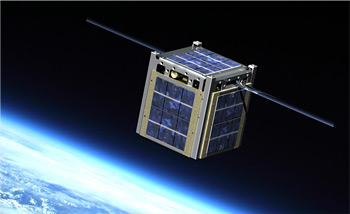
\includegraphics[width=0.8\linewidth]{./figs/cubesat_01}
			
		\begin{small}
			FONTE: \textit{NASA}\textsuperscript{\cite{NASA}}
		\end{small}		
	\end{figure}
		
	O \textit{CubeSat} Mauá, proposto no NSEE-IMT, é um equipamento do modelo 3U, sendo as unidades distribuídas em unidade de comunicação, unidade de controle de atitude e unidade de potência.
	
	\begin{figure}[th]
		\caption{ESTRUTURA DO CUBESAT PROPOSTA PELO NSEE-IMT}
		\centering
		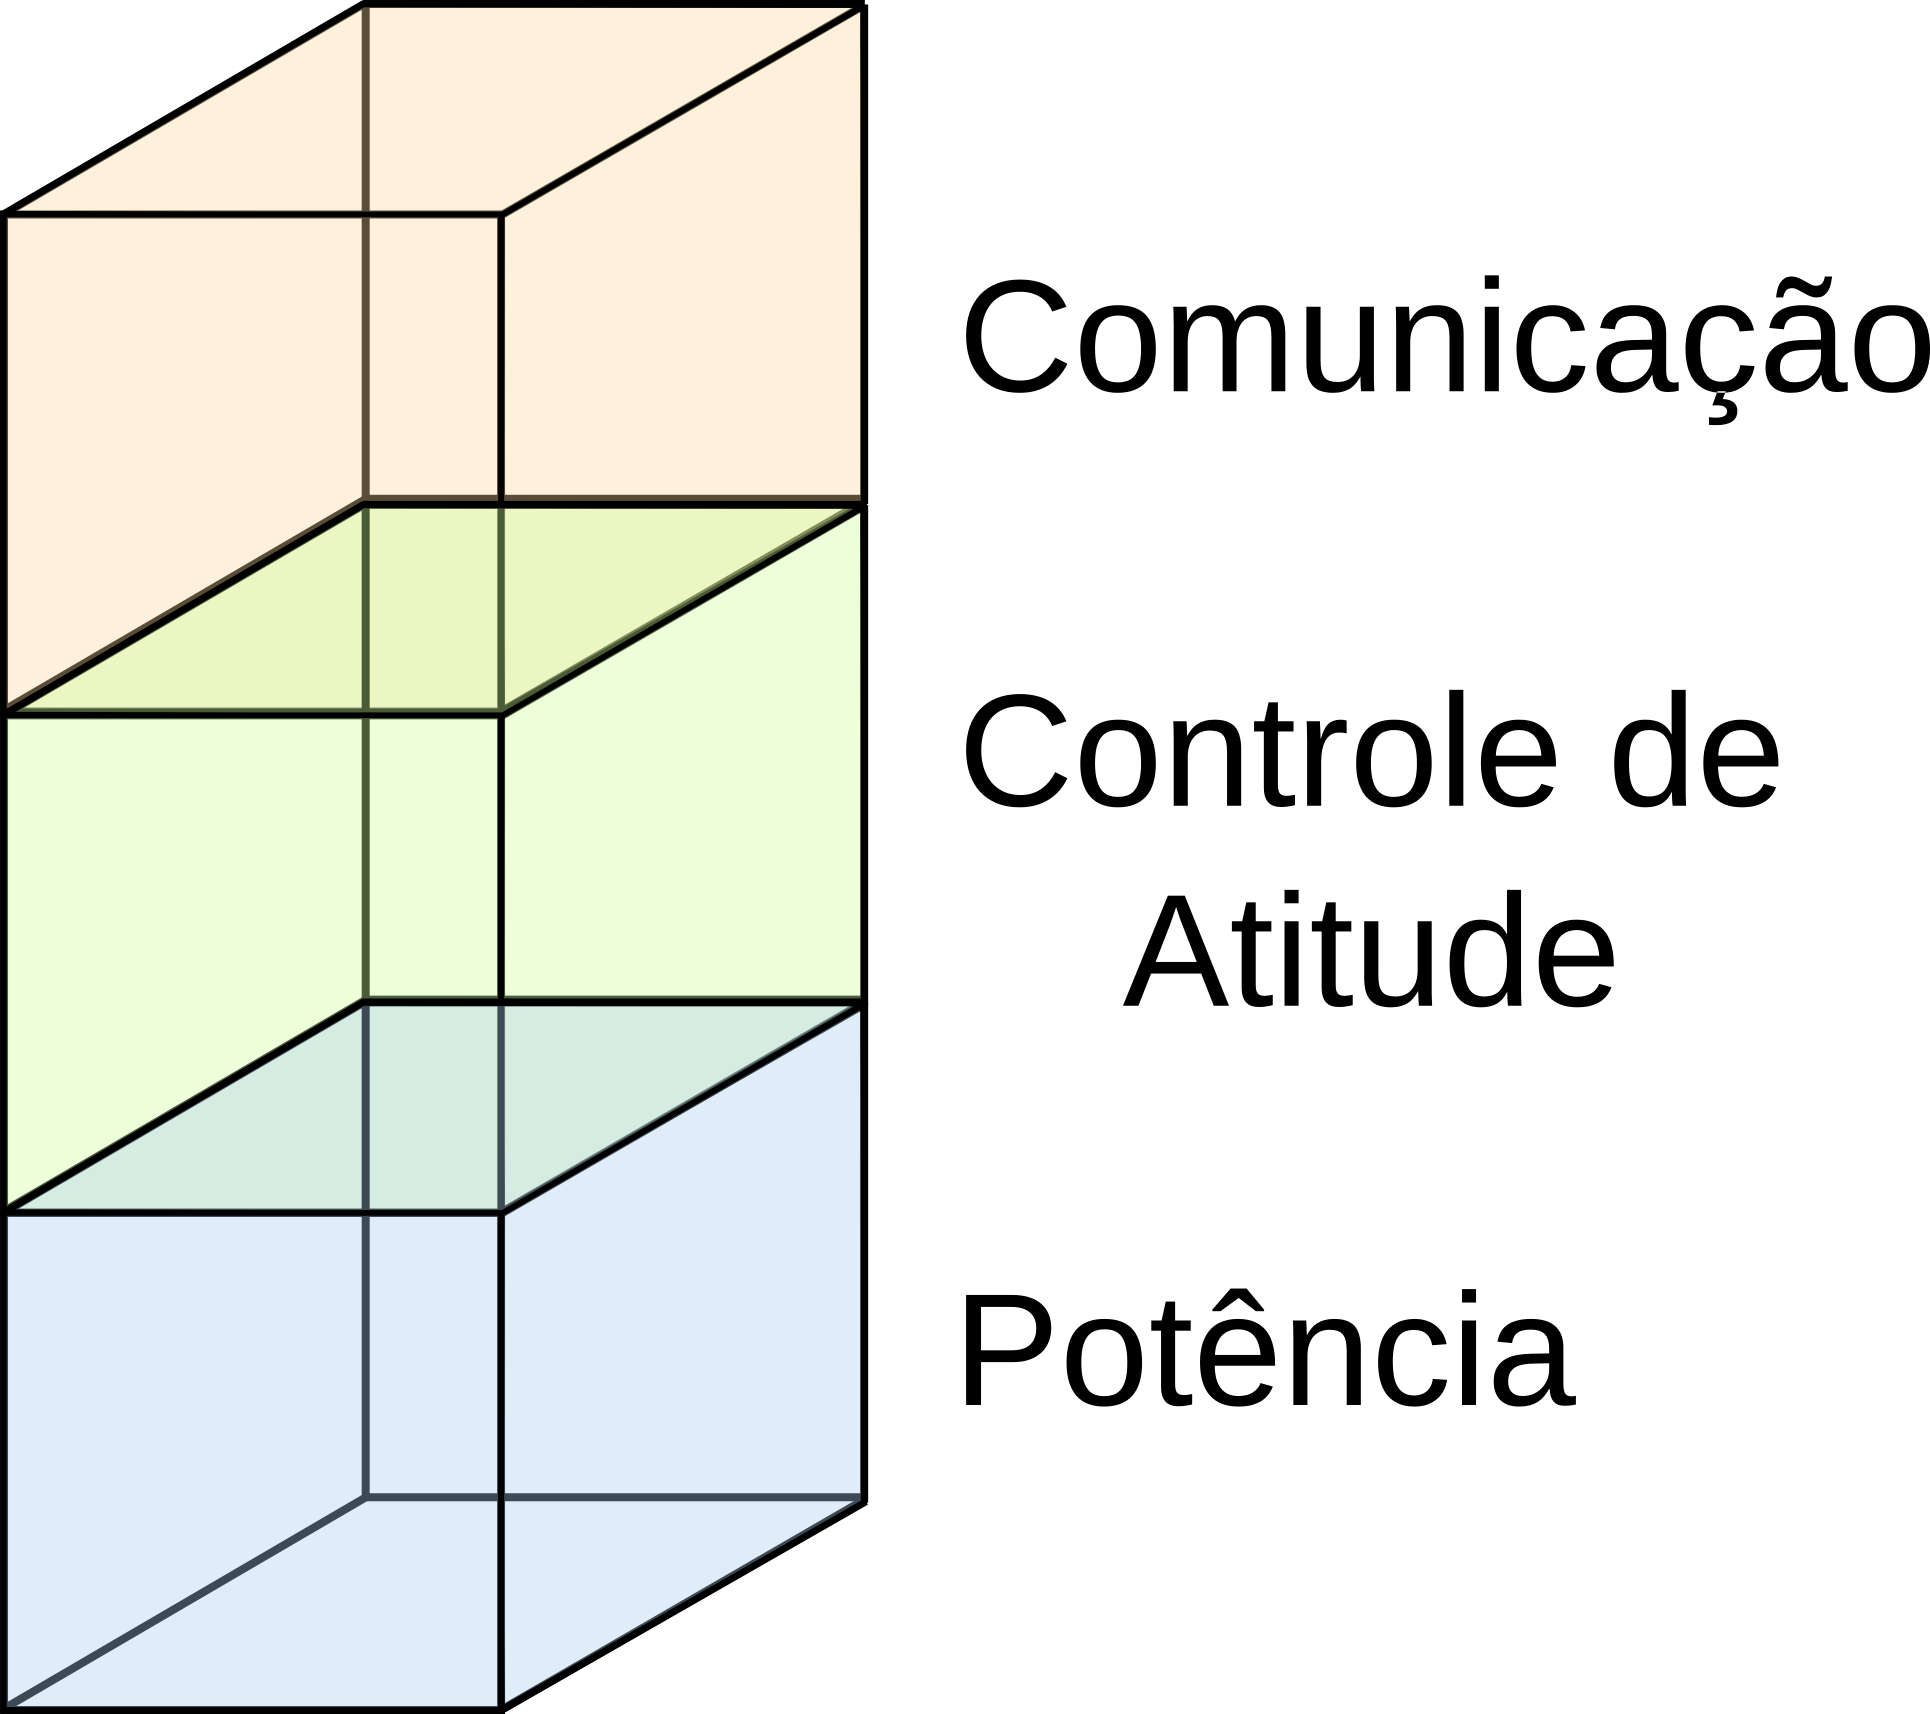
\includegraphics[width=0.4\linewidth]{./figs/cubesat_02}
			
		\begin{small}
			FONTE: Especificação do produto CubeSat\textsuperscript{\cite{Corsi}}
		\end{small}		
	\end{figure}
	\pagebreak

\section[Surgimento]{Surgimento} 

	O primeiro projeto de um \textit{CubeSat} foi proposto em 1999 pelos professores Jordi Puig-Suari, da \textit{California Polytechnic State University}, e Bob Twiggs, da \textit{Stanford University}. O objetivo do projeto foi o de padronizar o \textit{design} de picosatélites, visando a redução de custos e de tempo de desenvolvimento, além de prover uma maior acessibilidade ao espaço e conseguir realizar lançamentos frequentes, o que é de inviável obtenção com os satélites de grande porte.\textsuperscript{\cite{CubeSat}}

\section[No Brasil]{No Brasil}

	Os projetos de picosatélites, nanosatélites e microsatélites se multiplicam a cada ano, não só no Brasil mas em todo o mundo. A \textit{Cal Poly} estima que atualmente o projeto \textit{CubeSat} conte com a colaboração internacional de mais de 100 universidades, colégios e de algumas empresas e governos.
	
	Atualmente vários projetos nessa área, de pequenos satélites para diversas áreas da pesquisa científica e tecnológica, estão em curso no Brasil e outros ainda em fase de discussão, dentre eles se destacam os projetos abaixo:
	
	\begin{itemize}
		\item \textbf{Tancredo 1}
		
			Picosatélite desenvolvido pelo grupo do professor Cândido Moura da Escola Tancredo Neves de Ubatuba, São Paulo. Primeiro satélite do Projeto UbatubaSat.\textsuperscript{\cite{UbatubaSat}}
			
		\item \textbf{AESP-14}		
		
			Cubesat desenvolvido pelo grupo do Dr. Pedro Lacava, professor e coordenador do Curso de Engenharia Aeroespacial do Instituto Tecnológico de Aeronáutica (ITA).\textsuperscript{\cite{AESP14}}
			
		\item \textbf{NanoSatC-Br2}
		
			Nanosatélite em desenvolvimento pelo grupo coordenado pelo Dr. Nelson Schuch do Centro Regional Sul do INPE (CRS) e do Dr. Otávio Durão (INPE/SJC), em parceria com pesquisadores da Universidade Federal de Santa Maria (UFSM) do Rio Grande do Sul, em orbita desde 19/06/2014.\textsuperscript{\cite{INPE}}

		\item \textbf{14-BISat}

			Nanosatélite científico em desenvolvimento pelo grupo liderado pelo professor Cedric Salotto, coordenador do Centro de Referência em Sistemas Embarcados e Aeroespaciais (CRSEA) do Instituto Federal Fluminense (IFF) da cidade de Campos dos Goytacazes (RJ), em parceria com a empresa Tekever S/A e a Faculdade de Engenharia da Universidade do Porto (FEUP), Portugal. Este projeto faz parte da missão internacional QB50.\textsuperscript{\cite{IFF}}
			
		\item \textbf{ITASAT-1}	

			Nanosatélite tecnológico em desenvolvimento pelo grupo liderado pelo Major Eloi Fonseca, professor do Curso de Engenharia Aeroespacial do Instituto Tecnológico de Aeronáutica (ITA) em parceria com a Agência Espacial Brasileira (AEB), Instituto Nacional de Pesquisas Espaciais (INPE-SJC, INPE-CRN e INPE-SM), Universidade do Vale do Rio dos Sinos (UNISINOS), Universidade Federal do Rio Grande do Norte (UFRN) e Universidade Federal de Santa Maria (UFSM).\textsuperscript{\cite{ITASAT}}	
			
	\end{itemize}

	Nesse capítulo foram apresentadas as premissas básicas de um projeto de \textit{CubeSat}, assim como o seu surgimento e  um resumo do segmento de nanossatélites no Brasil.


% ----------------------------------------------------------
% Materiais e Método
% ----------------------------------------------------------
\chapter[Materiais e Método]{Materiais e Método}

	Para auxiliar no projeto, as atividades foram divididas de forma a trazer, além do ganho teórico, uma maior dinâmica no desenvolvimento do mesmo. Essa etapa do projeto visou a máxima aquisição de dados possível sobre o tema proposto, foram abertas distintas frentes de trabalho para agilizar a aquisição teórica. Além do conhecimento adquirido foram definidos os principais componentes e equipamentos que foram utilizados no protótipo, como por exemplo as baterias, fotocélulas, componentes passivos e semicondutores.
	
	Também foi possível identificar e conhecer, de forma mais profunda, possíveis testes que podem ser realizados no Sistema de Gerenciamento de Energia para \textit{CubeSat}, como os testes de radiação, temperatura e pressão. Esses testes são de extrema importância para a detecção de possíveis problemas que possam existir, pois uma vez que o \textit{CubeSat} for lançado nada mais poderá ser feito para reparar possíveis problemas.
	
% ----------------------------------------------------------
% Etapas
% ----------------------------------------------------------
\section[Condições do espaço]{Condições do espaço}
	
	Para o desenvolvimento do \textit{CubeSat} é de extrema importância ter conhecimento das condições de operação que o equipamento irá operar.
	
	Os \textit{CubeSats}, operam em órbita terrestre baixa (\textit{LEO - Low Earth Orbit}). A órbita \textit{LEO} é a órbita que se encontra abaixo de 2.000 km do nível do mar, os objetos que situam-se nela, geralmente, ficam entre 320 até 800 km da superfície terrestre, muito diferente dos satélites tradicionais que operam em órbita geoestacionária, cuja a distância é de 35.796 km em relação ao nível do mar.\textsuperscript{\cite{LEO}}\textsuperscript{\cite{GEO}}
	
	Satélites situados na órbita \textit{LEO} viajam em velocidades de aproximadamente 27.400 km/h ou 8 km/s, o que representa uma volta ao longo da Terra a cada 90 minutos. Já os satélites geoestacionários precisam ter uma velocidade que façam que eles acompanham sempre o mesmo ponto da Terra, por isso as velocidades deles são de aproximadamente 11.068 km/h ou 3 km/s. O planeta Terra tem uma velocidade de rotação de aproximadamente 1.669,8 km/h ou 0,5 km/s.\textsuperscript{\cite{LEO}}\textsuperscript{\cite{GEO}}
	
	 Outras características de destaque para a órbita \textit{LEO} são as condições de temperatura, variando de -170 ºC a 123 ºC e de pressão variando de 10\textsuperscript{-4} Pa a 10\textsuperscript{-6} Pa.\textsuperscript{\cite{LEO}}
	
	Órbitas inferiores a esta não apresentam muita estabilidade e são alvos de arrastamento atmosférico, que é a força de fricção que atua sobre o foguete ou satélite, cuja principal causa é a fricção entre as moléculas do ar e a superfície do foguete ou satélite.\textsuperscript{\cite{NASA2}}
	
	\begin{figure}[th]
		\caption{PRINCIPAIS TIPOS DE ÓRBITAS}
		\centering
		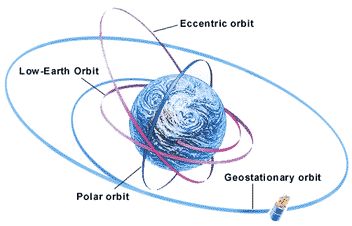
\includegraphics[width=0.5\linewidth]{./figs/cubesat_03}
			
		\begin{small}
			FONTE: Civil Air Patrol\textsuperscript{\cite{CAP}}
		\end{small}		
	\end{figure}	
	
	\pagebreak
	
	
\section[Definição dos componentes]{Definição dos componentes}

	A seguir será explicado de forma mais detalhada como foram realizadas as escolhas dos principais componentes do projeto. Importante ressaltar que os projetos de \textit{CubeSats} possuem como premissa o conceito de ser um projeto de baixo custo, porém o referencial do custo utilizado são os custos de projetos de grandes satélites.
	
	Para a utilização dos componentes que suportem as condições impostas  no meio espacial, alguns fabricantes possuem linhas de produtos voltadas para utilização de componentes aeroespaciais que possuem um custo mais elevado em comparação aos componentes utilizados no mercado comum.

\subsection[Bateria]{Bateria}

	
	As baterias têm a função principal de armazenar carga para poder assumir o controle do fornecimento de energia para todos os subsistemas do \textit{CubeSat}, nos momentos no qual o equipamento estiver situado em regiões de sombras solares, por exemplo atrás do planeta Terra. Nessas regiões, não há incidência de luz solar portanto as fotocélulas não irão gerar energia para o sistema. Dessa forma é preciso haver outro meio de geração de energia até que o \textit{CubeSat} volte a ter incidência de luz solar, caso contrário o sistema será desligado e o equipamento virará apenas lixo espacial.	
	
	Algumas das premissas básicas de projeto para a definição da bateria estão relacionadas com o seu poder de armazenamento de carga e o seu dimensional reduzido. Essas baterias ficaram alocadas no interior do \textit{CubeSat}, por isso a importância do dimensional reduzido, além disso não podem ser baterias com peso elevado, uma vez que a definição do projeto diz que os \textit{CubeSats} não podem ultrapassar 1,3 kg.
	
	Para a definição da bateria foi realizado um levantamento dos prós e contras dos tipos mais comuns de baterias encontradas no mercado, sendo elas de: níquel cádmio, hidreto metálico de níquel, íon-lítio e polímero de lítio.
		
	\begin{table}[th]
	\caption{TIPOS DE BATERIAS E AS PRINCÍPAIS CARACTERÍSTICAS}
	\begin{tabular}{p{4cm}|p{6cm}|p{5cm}}
	\textbf{Composição} & \textbf{Prós} & \textbf{Contras}\\
	\hline
	Níquel cádmio & Baixo custo & Tecnologia obsoleta, baixo ciclo de vida, possui efeito memória, altamente tóxica\\
	\hline
	Hidreto metálico de níquel (NiMH) &	Boa capacidade de armazenamento, ciclo de vida longo, rápida capacidade de carga, baixo desempenho, auto-descarga de 2\% ao dia & Efeito memória\\
	\hline
	Íon-lítio & Armazena mais carga do que as anteriores, não tem efeito memória, peso e volume reduzido, alto desempenho, alta densidade energética, ampla faixa de temperatura de operação, baixo tempo de carga, ciclo de vida longo & Inflamável, inutilidade em caso de descarga total\\
	\hline
	Polímero de lítio & Os mesmos da íon-lítio, alta taxa de descarga & Mais inflamável, inutilidade em caso de descarga total, alto custo\\	
	\hline
	\end{tabular}
	
	\begin{small}
	\vspace{3pt}
		FONTE: Elaborada pelos autores através de pesquisas realizadas na internet.
	\end{small}
	\end{table}
		
	Dentre os modelos comparados na Tabela 1, foi escolhida a bateria do tipo íon-lítio. Foram utilizadas duas baterias de duas células de 7,4 V e 2000 mAh, sendo uma para o conjunto principal e a outra para o conjunto de redundância do Sistema de Gerenciamento de Energia para \textit{CubeSat}. Na Figura 4, é possível visualizar a bateria selecionada.
	
	\begin{figure}[th]
		\caption{BATERIA DE ÍON-LÍTIO SELECIONADA}
		\centering
		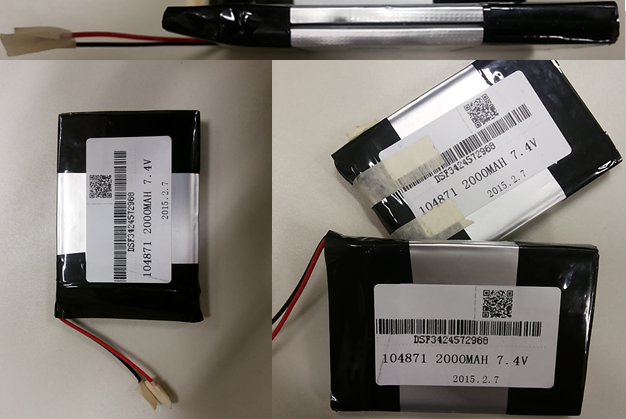
\includegraphics[width=0.6\linewidth]{./figs/cubesat_04}
			
		\begin{small}
			FONTE: Fotos tiradas pelos autores
		\end{small}
	\end{figure}
	
\subsubsection[Princípio de funcionamento]{Princípio de funcionamento}
	
	As baterias de íon-lítio, têm esse nome devido ao seu princípio de funcionamento o qual consiste no movimento dos íons de lítio (Li) que migram do ânodo para o cátodo por meio de um solvente não aquoso, conforme pode ser visto na Figura 5.\textsuperscript{\cite{BraEsc}}
	
	\begin{figure}[th]
		\caption{PRINCÍPIO DE FUNCIONAMENTO DA BATERIA DE ÍON-LÍTIO}
		\centering
		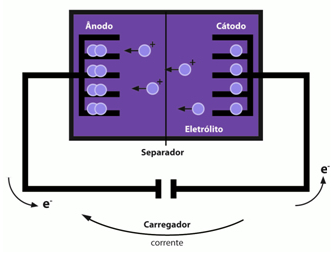
\includegraphics[width=0.6\linewidth]{./figs/cubesat_05}
			
		\begin{small}
			FONTE: Brasil Escola\textsuperscript{\cite{BraEsc}}
		\end{small}		
	\end{figure}

	O lítio (Li) é considerado o metal mais leve existente na Terra (desconsiderando os feitos em laboratório), por essa razão que as baterias de íon-lítio possuem baixo peso, o que é de fundamental importância para o projeto do \textit{CubeSat}. Por se tratar de um dos tipos de bateria mais comuns, sendo amplamente encontrado em \textit{smartphones} e \textit{notebooks}, acaba tendo um impacto positivo nos custos de aquisição das mesmas.\textsuperscript{\cite{TecMundo}}
	
\subsection[Fotocélulas]{Fotocélulas}

	As fotocélulas são fundamental importância para o sistema, uma vez que elas são as responsáveis pela captação da luz solar que irá gerar a energia necessária para o funcionamento do \textit{CubeSat}. É importante que elas possuam rendimento elevado, pois devido as condições impostas pela órbita \textit{LEO}, na qual o \textit{CubeSat} irá ficar um terço do período de translação em regiões de sombra, ou seja, estará sem a incidência direta de luz solar.
	
\subsubsection[Princípio de funcionamento]{Princípio de funcionamento}

	As fotocélulas são um exemplo de aplicação prática do efeito fotoelétrico, descoberto por Heinrich Rudolf Hertz, em 1887 e explicado por Albert Einstein, em 1905.\textsuperscript{\cite{celula}}
	
	Quando uma grande quantidade de fótons é incidida em uma fotocélula a energia é absorvida. Essa absorção de energia permite que os átomos dos elementos que constituem a célula liberem elétrons, o espaço liberado é preenchido por outro elétron de uma camada inferior do semicondutor. Essa movimentação de elétrons, faz com que um dos lados da célula tenha uma concentração maior de elétrons, o que origina a diferença de potencial entre os lados, conforme pode ser visto na Figura 6.\textsuperscript{\cite{celula2}}
	
	\begin{figure}[th]
		\caption{PRINCÍPIO DE FUNCIONAMENTO DE UMA FOTOCÉLULA}
		\centering
		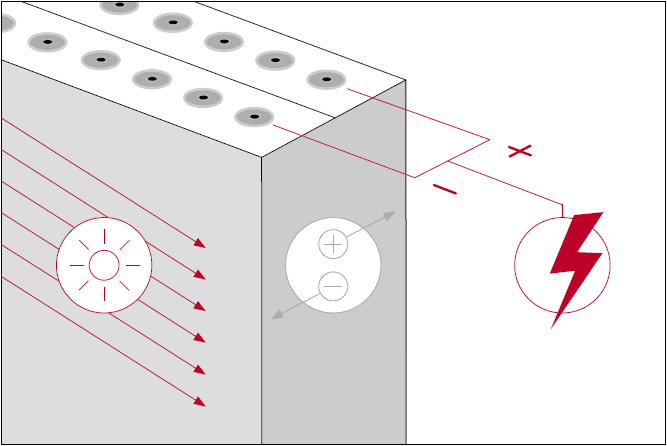
\includegraphics[width=0.6\linewidth]{./figs/fotocelula}
			
		\begin{small}
			FONTE: Sapa Solar\textsuperscript{\cite{celula2}}
		\end{small}		
	\end{figure}

\subsubsection[VIS Technology]{\textit{VIS Technology}}
	
	Inicialmente foi indicado pelo Engenheiro Rafael Corsi, do NSEE-IMT, o contato da empresa \textit{Vis Technology}, um empresa nacional, localizada em São Paulo, que desenvolve projetos com energias renováveis. Porém as fotocélulas utilizadas por eles são para aplicações industriais. Essas fotocélulas possuem um rendimento entre 10\% e 12\%, muito abaixo comparado ao rendimento com as próprias de aplicações aeroespaciais, além de terem um dimensional maior, conforme pode ser visualizado na Figura 7.
	
	\begin{figure}[th]
		\caption{FOTOCÉLULAS DA \textit{VIS TECHNOLOGY}}
		\centering
		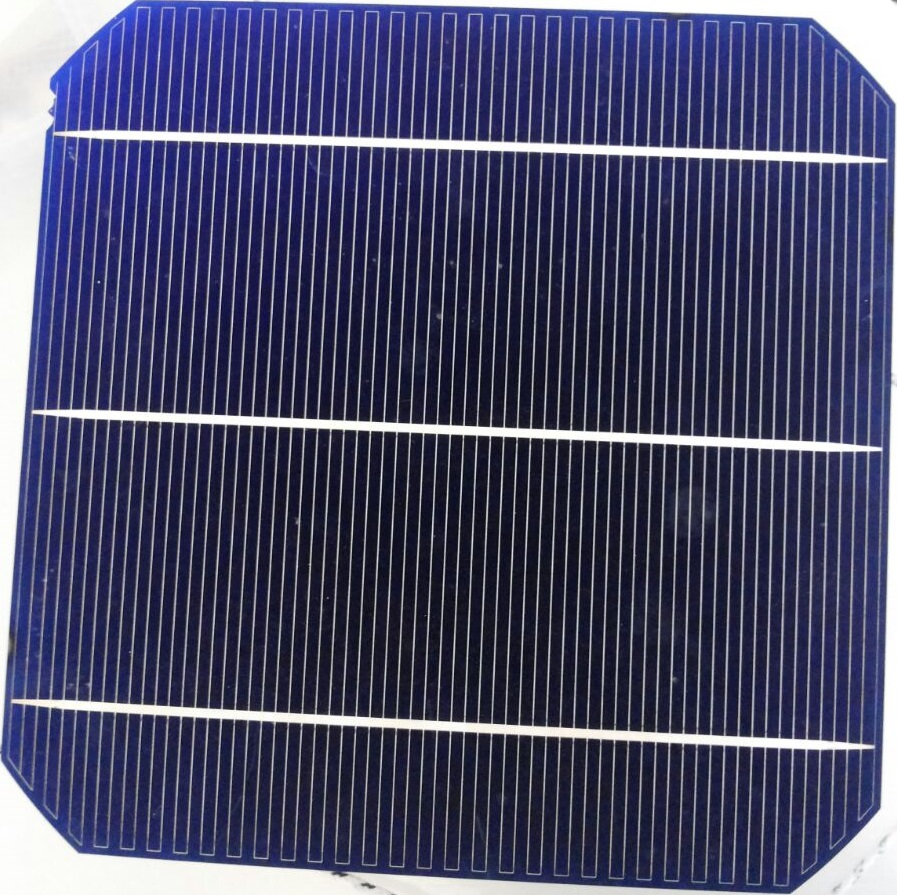
\includegraphics[width=0.3\linewidth]{./figs/cell_vis}
			
		\begin{small}
			FONTE: Foto tirada pelos autores
		\end{small}		
	\end{figure}
	\pagebreak
	
	Mesmo sabendo dessas limitações, foram obtidas algumas amostras. Essas amostras serviram para um primeiro contato com essa tecnologia, conseguindo realizar alguns ensaios a fim de se obter uma familiaridade maior com o componente, conforme pode ser visto na Figura 8.
	
	\begin{figure}[th]
		\caption{\textit{SET UP} PARA TESTE DAS FOTOCÉLULAS DA \textit{VIS TECHNOLOGY}}
		\centering
		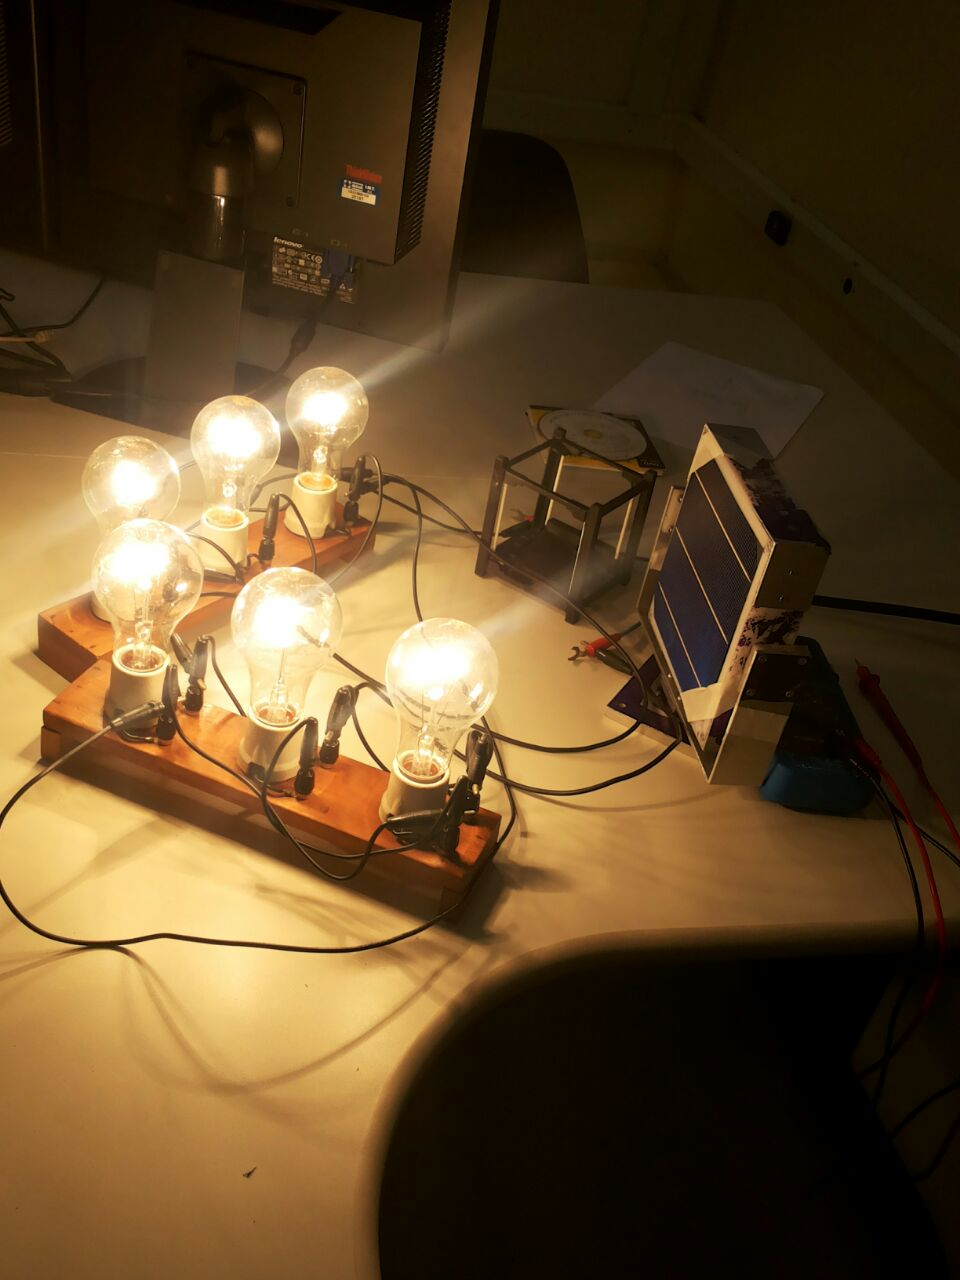
\includegraphics[width=0.4\linewidth]{./figs/setup}
			
		\begin{small}
			FONTE: Foto tirada pelos autores
		\end{small}		
	\end{figure}
	
	Após uma breve familiarização com as fotocélulas, foram analisados diversos projetos de \textit{CubeSats} e identificados os principais fornecedores de fotocélulas (\textit{SpectroLab}, \textit{Emcore} e \textit{AzurSpace Solar}) para aplicações aeroespaciais.
	
	Foi realizado um estudo apurado dos principais tipos de fotocélulas disponíveis nos portfólios desses fornecedores, visando identificar os modelos que se melhor ajustavam no desenvolvimento do \textit{CubeSat}.
	
\subsubsection[SpectroLab]{\textit{SpectroLab}}
	
	A \textit{SpectroLab}, empresa subsidiária da \textit{The Boeing Company}, é a fabricante líder mundial de células solares de multi-junção de alta eficiência e de painéis solares. A empresa é sediada nos Estados Unidos, mais especificamente em Los Angeles, Califórnia.\textsuperscript{\cite{SpectroLab}}
	
	\begin{table}[th]
	\caption{COMPARATIVO DAS FOTOCÉLULAS DA \textit{SPECTROLAB}}
	\begin{tabular}{p{2.5cm}|p{3.1cm}|p{3.1cm}|p{3.1cm}|p{3.1cm}}
		\textbf{Modelo} & \textit{\textbf{PV UTJ Cell}} & \textit{\textbf{PV XTJ Cell}} & \textit{\textbf{PV NM TASC ITJ}} & \textit{\textbf{PV ITJ Cell}} \\
		\hline
		\textbf{Rendimento} & 28,3\% & 29,5\% & 24\% a 30\% & 26,8\% \\
		\hline
		\textbf{Material} & GaInP2/GaAs/Ge & GaInP2/GaAs/Ge & GaInP2/GaAs/Ge & GaInP2/GaAs/Ge\\
		\hline
		\textbf{Tensão} & 2,660 V & 2,633 V & 2,520 V & 2,565 V\\
		\hline
		\textbf{Corrente} & 454 mA & 472 mA & 31 mA & 441 mA\\
		\hline
		\textbf{Dimensional} & 26,62 cm\textsuperscript{2} & 26,62 cm\textsuperscript{2} & 2,277 cm\textsuperscript{2} & 31 cm\textsuperscript{2}\\
		\hline
		\textbf{Peso} & 84 mg/cm\textsuperscript{2} & 84 mg/cm\textsuperscript{2} & 0,234 g & 84 mg/cm\textsuperscript{2}\\
	\end{tabular}
	
	\begin{small}
	\vspace{3pt}
		FONTE: Elaborada pelos autores através de informações coletadas nos \textit{datasheets} dos produtos.
	\end{small}
	\begin{footnotesize}
		NOTA: Condições de teste: \textit{AM} 0, \textit{WRC} = 135,3 mW/cm\textsuperscript{2}, T = 28ºC.
	\end{footnotesize}
	\end{table}
	
	Avaliando os dados da Tabela 2, os modelos \textit{PV UTJ Cell} e \textit{PV XTJ Cell}, foram os mais indicados para a aplicação, devido ao alto rendimento (superior a 28\%) apresentado
	
	\begin{figure}[th]
		\caption{MODELO DE FOTOCÉLULA DA \textit{SPECTROLAB}}
		\centering
		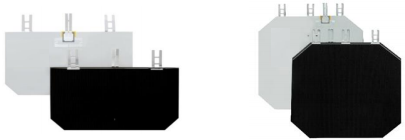
\includegraphics[width=1.0\linewidth]{./figs/UTJ}
			
		\begin{small}
			FONTE: \textit{SpectroLab}\textsuperscript{\cite{SpectroLab2}}
		\end{small}		
	\end{figure}

\subsubsection[Emcore]{\textit{Emcore}}

	Em dezembro de 2014, a \textit{Emcore} foi comprada pela \textit{SolAero Technologies}, que é uma das fabricantes líderes mundial de alta eficiência, células solares e painéis solares para aplicações espaciais. Assim como a \textit{SpectroLab}, está sediada nos Estados Unidos, porém no município de Albuquerque, Novo México.\textsuperscript{\cite{Emcore}}\textsuperscript{\cite{Emcore2}}
	
	\begin{table}[th]
	\caption{COMPARATIVO DAS FOTOCÉLULAS DA \textit{EMCORE}}
	\begin{tabular}{p{2.5cm}|p{3.1cm}|p{3.1cm}|p{3.1cm}|p{3.1cm}}
		\textbf{Modelo} & \textit{\textbf{ATJ PV Cell}} & \textit{\textbf{BTJ PV Cell}} & \textit{\textbf{BTJM PV Cell}} & \textit{\textbf{ZTJ PV Cell}} \\
		\hline
		\textbf{Rendimento} & 27,5\% & 28,5\% & 28\% & 29,5\% \\
		\hline
		\textbf{Material} & GaInP/GaAs/Ge & GaInP/GaAs/Ge & GaInP/GaAs/Ge & GaInP/GaAs/Ge\\
		\hline
		\textbf{Tensão} & 2,60 V & 2,70 V & 2,69 V & 2,73 V\\
		\hline
		\textbf{Corrente} & 454 mA & 455 mA & 454 mA & 467 mA\\
		\hline
		\textbf{Dimensional} & 26,6 cm\textsuperscript{2} & 26,6 cm\textsuperscript{2} & 26,6 cm\textsuperscript{2} & 26,6 cm\textsuperscript{2}\\
		\hline
		\textbf{Peso} & 84 mg/cm\textsuperscript{2} & 84 mg/cm\textsuperscript{2} & 84 mg/cm\textsuperscript{2} & 84 mg/cm\textsuperscript{2}\\
	\end{tabular}
	
	\begin{small}
	\vspace{3pt}
		FONTE: Elaborada pelos autores através de informações coletadas nos \textit{datasheets} dos produtos.
	\end{small}
	\begin{footnotesize}
		NOTA: Condições de teste: \textit{AM} 0, \textit{WRC} = 135,3 mW/cm\textsuperscript{2}, T = 28ºC.
	\end{footnotesize}
	\end{table}
	
	Avaliando os dados da Tabela 3, os modelos \textit{BTJ PV Cell}, \textit{BTJM PV Cell} e \textit{ZTJ PV Cell}, foram os mais indicados para a aplicação, devido ao alto rendimento (superior a 28\%) apresentado.
	
	\begin{figure}[th]
		\caption{MODELO DE FOTOCÉLULA DA \textit{EMCORE}}
		\centering
		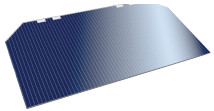
\includegraphics[width=0.5\linewidth]{./figs/ZTJ}
			
		\begin{small}
			FONTE: \textit{SolAero Technologies}\textsuperscript{\cite{Emcore3}}
		\end{small}		
	\end{figure}
	
\subsubsection[AzurSpace]{\textit{AzurSpace}}

	A \textit{AzurSpace} é a líder européia no desenvolvimento e produção de células solares multi-junção para aplicações espaciais e terrestres, com quase 50 anos de experiência no mercado. A empresa localiza-se em Heilbronn, cidade em Baden-Württemberg, Alemanha.\textsuperscript{\cite{AzurSpace}}
	
	\begin{table}[th]
	\caption{COMPARATIVO DAS FOTOCÉLULAS DA \textit{AZURSPACE}}
	\begin{tabular}{p{2.5cm}|p{3.1cm}|p{3.1cm}|p{3.1cm}|p{3.1cm}}
		\textbf{Modelo} & \textit{\textbf{3G30C}} & \textit{\textbf{3G30C-Large}} & \textit{\textbf{3G30C-Large-120x60}} & \textit{\textbf{3G28C}} \\
		\hline
		\textbf{Rendimento} & 30\% & 30\% & 30\% & 28\% \\
		\hline
		\textbf{Material} & GaInP/GaAs/Ge & GaInP/GaAs/Ge & GaInP/GaAs/Ge & GaInP/GaAs/Ge\\
		\hline
		\textbf{Tensão} & 2,700 V & 2,700 V & 2,700 V & 2,667 V\\
		\hline
		\textbf{Corrente} & 520,2 mA & 1041 mA & 1186 mA & 506 mA\\
		\hline
		\textbf{Dimensional} & 30,18 cm\textsuperscript{2} & 60,36 cm\textsuperscript{2} & 68,76 cm\textsuperscript{2} & 30,18 cm\textsuperscript{2}\\
		\hline
		\textbf{Peso} & 86 mg/cm\textsuperscript{2} & 114 mg/cm\textsuperscript{2} & 130 mg/cm\textsuperscript{2} & 86 mg/cm\textsuperscript{2}\\
	\end{tabular}
	
	\begin{small}
	\vspace{3pt}
		FONTE: Elaborada pelos autores através de informações coletadas nos \textit{datasheets} dos produtos.
	\end{small}
	\begin{footnotesize}
		NOTA: Condições de teste: \textit{AM} 0, \textit{WRC} = 1367 W/m\textsuperscript{2}, T = 28ºC.
	\end{footnotesize}
	\end{table}	
	
	Avaliando os dados da Tabela 4, os modelos \textit{30G28C} e \textit{30G30C}, foram os mais indicados para a aplicação, devido ao alto rendimento (superior a 28\%) apresentado. Os demais modelos não atenderam o dimensionamento adequado para o projeto.
	
	\begin{figure}[th]
		\caption{MODELO DE FOTOCÉLULA DA \textit{AZURSPACE}}
		\centering
		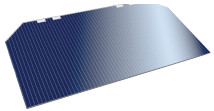
\includegraphics[width=0.5\linewidth]{./figs/ZTJ}
			
		\begin{small}
			FONTE: \textit{AzurSpace}\textsuperscript{\cite{AzurSpace2}}
		\end{small}		
	\end{figure}	
	\pagebreak
	
\subsubsection[Análise de preços]{Análise de preços}

	Selecionados os modelos dos principais fornecedor, foi solicitado um orçamento das fotocélulas para realizar o comparativo dos preços e, por fim, realizar os procedimentos necessários para a aquisição das mesmas.
	
	O contato com a \textit{SpectroLab} não teve obteve sucesso, uma vez que a empresa não respondeu nenhuma das tentativas de contato realizadas. Já a solicitação do orçamento da \textit{SolAero Technologies} (antiga \textit{Emcore}) não caminhou conforme esperado, uma vez que uma das políticas de vendas da empresa é de um pedido mínimo de \$7.500,00 dólares.
	
	A \textit{AzurSpace} enviou um orçamento dos modelos solicitados, conforme Tabela 5.
	
	\begin{table}[th]
	\caption{ORÇAMENTO DAS FOTOCÉLULAS DA \textit{AZURSPACE}}
	\centering
	\begin{tabular}{p{3.0cm}|p{3.0cm}|p{3.0cm}|p{3.0cm}}
		\textbf{Modelo} & \textbf{Valor unitário} & \textbf{Frete} & \textit{\textbf{Lead time}}\\
		\hline
		3G28C & \euro 193,00 & \euro 195,00 & 8 a 10 semanas\\
		3G30C & \euro 198,00 & \euro 195,00 & 8 a 10 semanas\\

	\end{tabular}
	
	\begin{small}
	\vspace{3pt}
		FONTE: Elaborada pelos autores através do orçamento recebido pela \textit{AzurSpace}
	\end{small}
	\end{table}	
	
\subsubsection[TrisolX]{TrisolX}	
	
	Devido ao alto custo e o grande \textit{lead time} da \textit{AzurSpace}, novas pesquisas foram feitas na tentativa de encontrar um novo fornecedor de fotocélulas com um custo mais acessível. Após uma busca detalhada em diversos grupos de discussões sobre o desenvolvimento de \textit{CubeSats}, foi encontrada no \textit{LinkedIn} a empresa \textit{TrisolX}.
	
	A \textit{TrisolX} é uma pequena empresa, localizada em Nova Iorque, que oferece uma alternativa acessível para projetos com orçamentos reduzidos. A empresa, vende a \textit{TrisolX Solar Wings}, que são fotocélulas cortadas a partir do modelo \textit{3G28C} da \textit{AzurSpace}.
	
	É o mesmo produto da \textit{AzurSpace}, porém com tamanho e formato diferentes, conforme Figura 12.
	
	\begin{figure}[th]
		\caption{MODELO DE FOTOCÉLULA DA \textit{TRISOLX}}
		\centering
		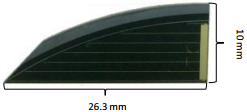
\includegraphics[width=0.5\linewidth]{./figs/TrisolX}
			
		\begin{small}
			FONTE: \textit{TrisolX}\textsuperscript{\cite{TrisolX}}
		\end{small}		
	\end{figure}	

	Foi solicitado um orçamento à \textit{TrisolX}, que prontamente foi recebido conforme Tabela 6.
	
	\begin{table}[th]
	\caption{ORÇAMENTO DAS FOTOCÉLULAS DA \textit{TRISOLX}}
	\centering
	\begin{tabular}{p{3.5cm}|p{2.5cm}|p{1.5cm}|p{1.5cm}|p{2.0cm}}
		\textbf{Pacote} & \textbf{Quantidade} & \textbf{Valor} & \textbf{Frete} & \textbf{Prazo de entrega}\\
		\hline
		\textit{Sample Pack} & 5 células & \$25,00 &  \$68,00 & 2 semanas\\
		\textit{Starter Pack} & 25 células & \$100,00 &  \$68,00 & 2 semanas\\
		\textit{Development Pack} & 100 células & \$400,00 & \$68,00 & 2 semanas\\
	\end{tabular}
	
	\begin{small}
	\vspace{3pt}
		FONTE: Elaborada pelos autores através do orçamento recebedido pela \textit{TrisolX}.
	\end{small}
	
	\begin{footnotesize}
		NOTA: O modelo das fotocélulas comercializado pela \textit{TrisolX} é o \textit{3G28C} da \textit{AzurSpace}.
	\end{footnotesize}
	\end{table}	
	
	Tendo como objetivo inicial fazer a validação do sistema como um todo, realizar testes de pressão, temperatura e radiação, para fazer um levantamento completo do funcionamento do sistema, foi solicitado para a \textit{TrisolX} o \textit{Starter Pack}. Dessa forma foi possível ganhar experiência no manuseio das fotocélulas e validar o sistema, para depois fazer a aquisição das fotocélulas mais robustas da \textit{AzurSpace}.
	
\subsection[Componentes passivos]{Componentes passivos}

	Os componentes passivos, são os componentes eletrônicos que não aumentam a intensidade da tensão ou da corrente de um circuito eletrônico, ou seja, são os resistores, indutores, capacitores e memristores.\textsuperscript{\cite{Passivo}} No desenvolvimento do projeto não foram utilizados os memristores.
	
	Resistores são componentes utilizados para controlar a intensidade da corrente elétrica que passa no circuito. Capacitores são componentes que armazenam e liberam cargas elétricas por meio da tensão elétrica. Indutor são componentes que utilizam o magnetismo para armazenar e liberar cargas por meio da corrente elétrica.

	É de extrema importância que os componentes passivos atendam algumas premissas para a utilização no projeto. Esses componentes precisam possuir uma grande faixa de temperatura de operação, uma certa tolerância a radiação e um dimensional pequeno (\textit{SMD}).
	
	Os capacitores, devido as baixas pressões encontradas no espaço, não podem ser do modelo eletrolítico, ou seja, precisam ser ou cerâmicos ou de tântalo. Os capacitores cerâmicos geralmente são de 0,5 pF até 470 nF com tensão de isolação de 25 V ou 50 V. Para esses capacitores tomou-se o cuidado de selecionar os capacitores com o coeficiente de temperatura X7R, devido a sua grande faixa de temperatura de operação, conforme indicado na Figura 13.\textsuperscript{\cite{x7r}}
	
	\begin{figure}[th]
		\caption{COEFICIENTES DE TEMPERATURA DOS CAPACITORES CERÂMICOS}
		\centering
		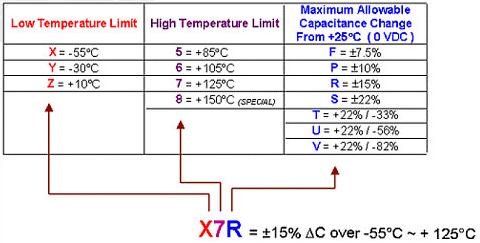
\includegraphics[width=0.8\linewidth]{./figs/x7r}
			
		\begin{small}
			FONTE: PY2BBS\textsuperscript{\cite{x7r}}
		\end{small}		
	\end{figure}	
	\pagebreak
	Além dessa característica, os capacitores X7R apresentam um bom comportamento com a variação de temperatura, comparado com os capacitores Y5V (outro modelo amplamente encontrado no mercado), conforme pode ser visto na Figura 14.
	
	\begin{figure}[th]
		\caption{VARIAÇÃO DA CAPACITÂNCIA EM FUNÇÃO DA TEMPERATURA}
		\centering
		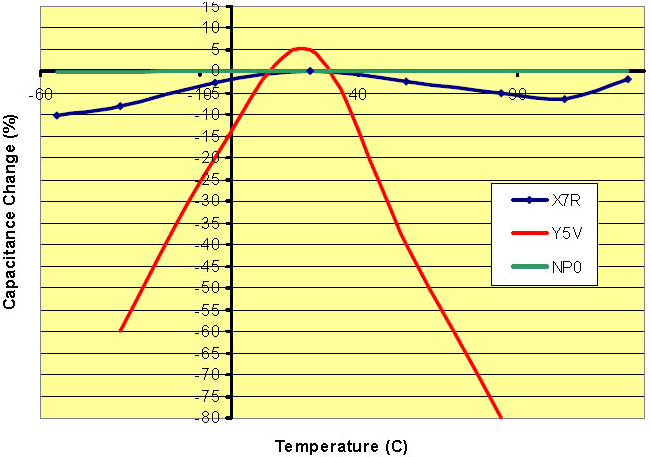
\includegraphics[width=0.8\linewidth]{./figs/y5v}
			
		\begin{small}
			FONTE: Johanson Dielectrics\textsuperscript{\cite{y5v}}
		\end{small}		
	\end{figure}
	
	Já os capacitores de tântalo apresentam valores de 0,22 pF até 100 $\mu$F, esse tipo de capacitor possui baixa corrente de fuga e baixas perdas, além de uma vida útil maior comparado aos eletrolíticos.\textsuperscript{\cite{x7r}}

\subsection[Semicondutores]{Semicondutores}

\subsection[Lista de componentes]{Lista de componentes}

	Seguindo as premissas apresentadas anteriormente, foi finalizada a lista de componentes necessárias para o seguimento do projeto, também foi levado em consideração a questão financeira, portanto alguns componentes apresentados nessa lista podem ser substituídos após a realização de todos os ensaios e validações.
	
	Na Figura 15 é possível visualizar a lista de componentes eletrônicos definida pelo grupo.
	
	\begin{figure}[th]
		\caption{LISTA DE COMPONENTES ELETRÔNICOS}
		\centering
		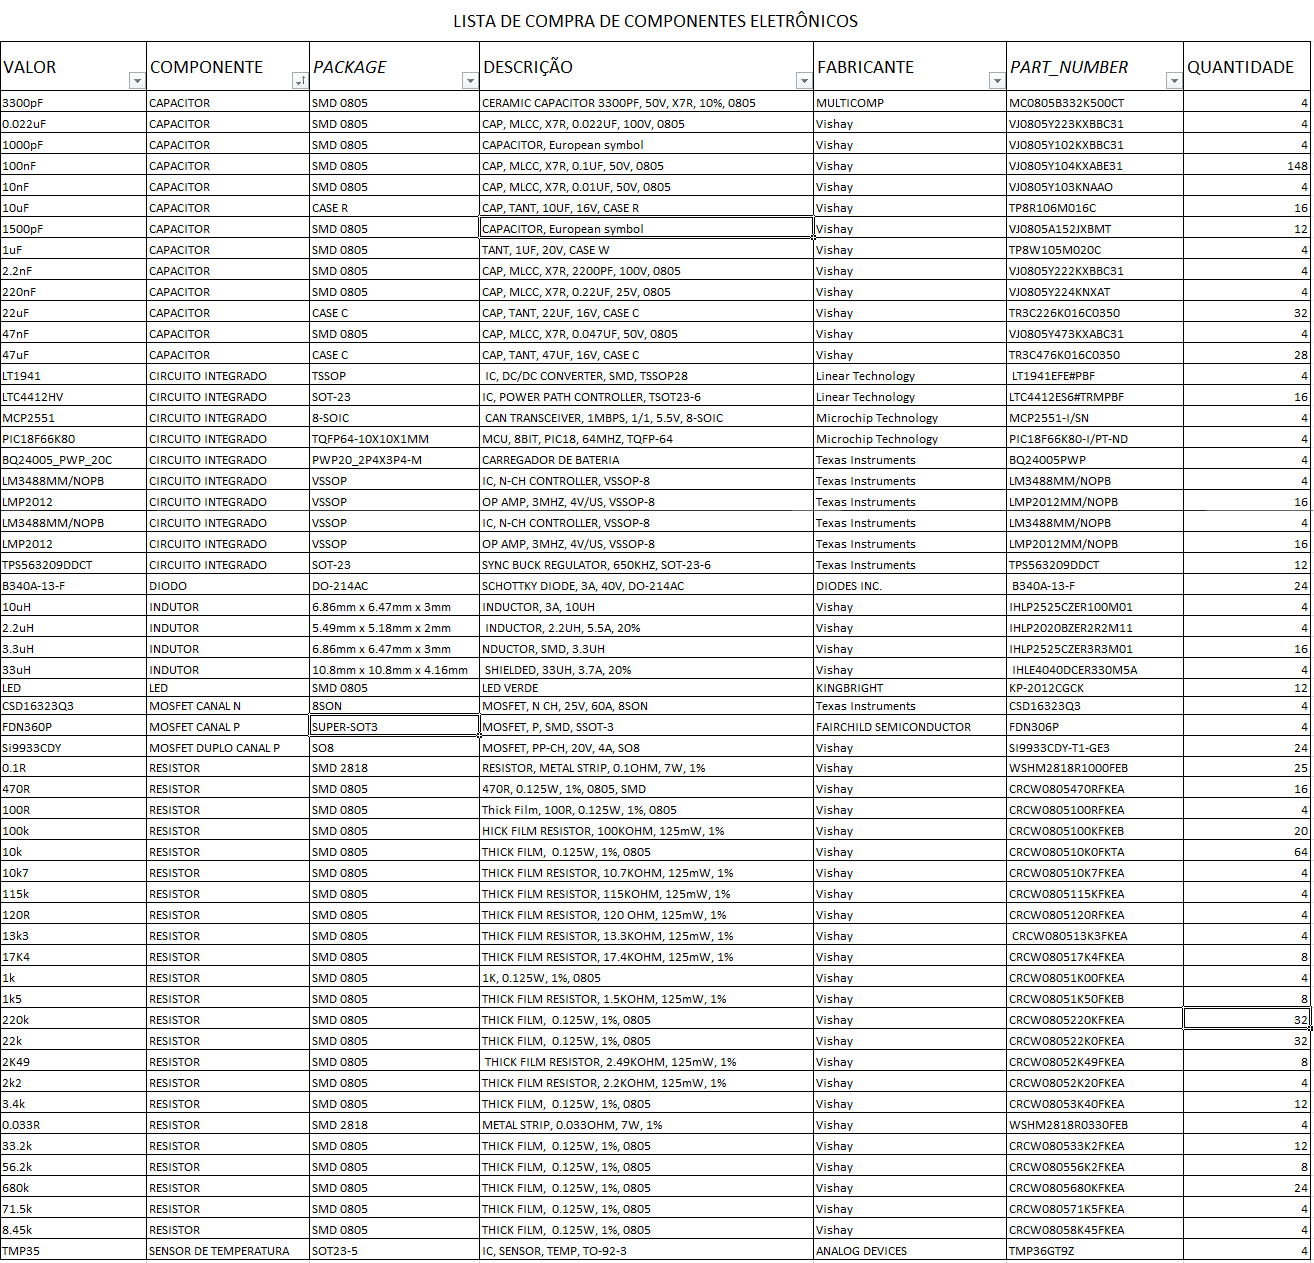
\includegraphics[width=1.0\linewidth]{./figs/comp}
			
		\begin{small}
			FONTE: Elaborado pelos autores.
		\end{small}		
	\end{figure}
	\pagebreak
	
	Foi solicitado um orçamento para a \textit{Farnell}, uma vez que o Instituto Mauá de Tecnologia tem a preferência de trabalhar com esse parceiro. O valor do orçamento, que tinha a disposição praticamente todos os componentes necessários com exceção do carregador de bateria (BQ24005PWP), ficou R\$ 2.065,66, conforme pode ser visto no Anexo A.
	

\section[Ensaios possíveis]{Ensaios possíveis}
	
	Durante a fase de aquisição teórica foram identificados possíveis ensaios que poderiam ser feitos no sistema para validação do circuito como um todo. Esses ensaios são de essencial importância para o projeto, pois dessa forma podem ser identificados possíveis problemas que devem ser corrigidos antes do lançamento da missão.
	
\subsection[Validação dos subconjuntos]{Validação dos subconjuntos}

	Um dos ensaios identificados foi o de validação dos subconjuntos do Sistema de Gerenciamento de Energia para \textit{CubeSat}. O circuito do sistema como um todo foi dividido em vários subconjuntos de funções especificas para serem validados, ou seja, foi separada a parte do carregador de bateria, do conversor 3,3 V, do conversosr de 5 V, do conversosr de 12 V e do conversor \textit{backup}. Na Figura 16 pode ser visualizado um dos subconjuntos do sistema.
	
	\begin{figure}[th]
		\caption{CIRCUITOS DOS SUBCONJUNTOS DO SISTEMA}
		\centering
		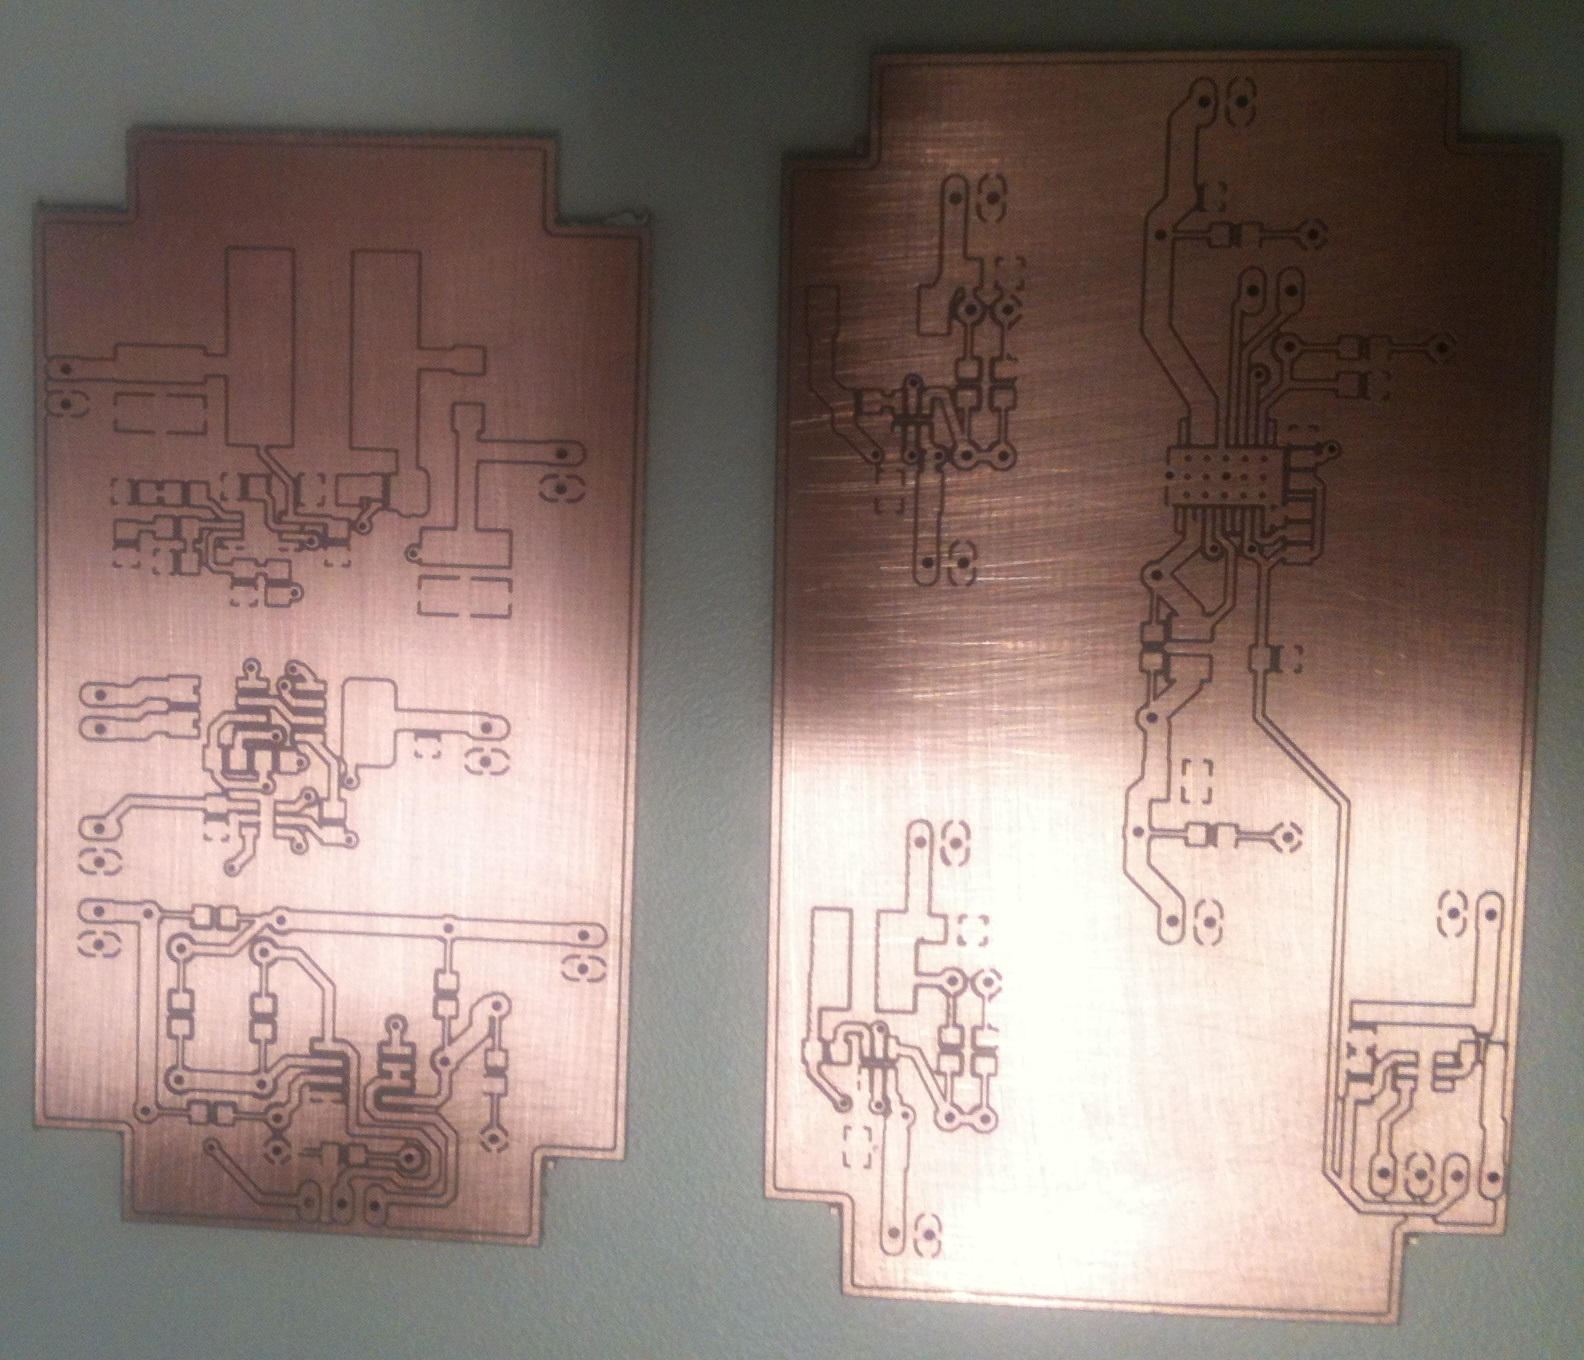
\includegraphics[width=0.5\linewidth]{./figs/placas_subconjuntos}
			
		\begin{small}
			FONTE: Fotos tiradas pelos autores.
		\end{small}		
	\end{figure}
	
\subsection[Ensaio de radiação]{Ensaio de radiação}	

	O ensaio de radiação consiste na emissão de radiação nos semicondutores a fim de se obter a assinatura da tensão e corrente após a exposição a radiação. Para esse ensaio foi necessário que os semicondutores estivessem decapados, ou seja, é necessário que a eletrônica do semicondutor esteja visível para que a emissão da radiação seja direta no componente, fato que não ocorrerá no espaço, uma vez que a película do componente estará presente o que, por sua vez, acaba dando uma pequena filtrada na radiação. Esse teste foi realizado em conjunto com o Centro Universitário da Faculdade de Engenharia Industrial (FEI), com a professora Marcilei da FEI.
	
	Entre diversas pesquisas a respeito de possíveis testes de radiação, foi encontrado o projeto \textit{Open Source Satellite Initiative}\textsuperscript{\cite{OSSI}}. Na \textit{wikipage}\textsuperscript{\cite{OSSI2}} do projeto \textit{OSSI} é disponibilizado um \textit{link} para um \textit{data base} que contém dados de testes de radiação da \textit{NASA Goddard Space Flight Center}.\textsuperscript{\cite{OSSI3}}
	
\subsection[Ensaio térmico]{Ensaio térmico}

\subsection[Ensaio de vácuo]{Ensaio de vácuo}	

\subsection[Ensaio de termovácuo]{Ensaio de termovácuo}		
	
	
	
	
% ----------------------------------------------------------
% PROTÓTIPO 
% ----------------------------------------------------------
\chapter[Protótipo]{Protótipo}

% ----------------------------------------------------------
% RESULTADOS E DISCUSSÕES
% ----------------------------------------------------------
\chapter[Resultados e discussões]{Resultados e discussões}

% ----------------------------------------------------------
% PLANO DE MARKETING
% ----------------------------------------------------------
\chapter[Plano de marketing]{Plano de marketing}

% ----------------------------------------------------------
% PLANO OPERACIONAL
% ----------------------------------------------------------
\chapter[Plano operacional]{Plano operacional}

% ----------------------------------------------------------
%PLANILHA FINANCEIRA 
% ----------------------------------------------------------
\chapter[Planilha financeira]{Planilha financeira}

% ----------------------------------------------------------
% CONCLUSÕES
% ----------------------------------------------------------
\chapter[Conclusões]{Conclusões}


% ----------------------------------------------------------
% REFERÊNCIAS BIBLIOGRÁFICAS
% ----------------------------------------------------------
\bibliography{TCC_Sist_Gerenciamento_Potencia}

% ----------------------------------------------------------
% Anexos
% ----------------------------------------------------------

% ---
% Inicia os anexos
% ---
\begin{anexosenv}

% Imprime uma página indicando o início dos anexos
\partanexos

% ---
\chapter[Orçamento dos componentes da Farnell]{Orçamento dos componentes da \textit{Farnell}}
% ---

Orçamento enviado pelo Sr. Helder Sant'ana Viana da \textit{Farnell Newark element14}.

	\begin{figure}[th]
		\centering
		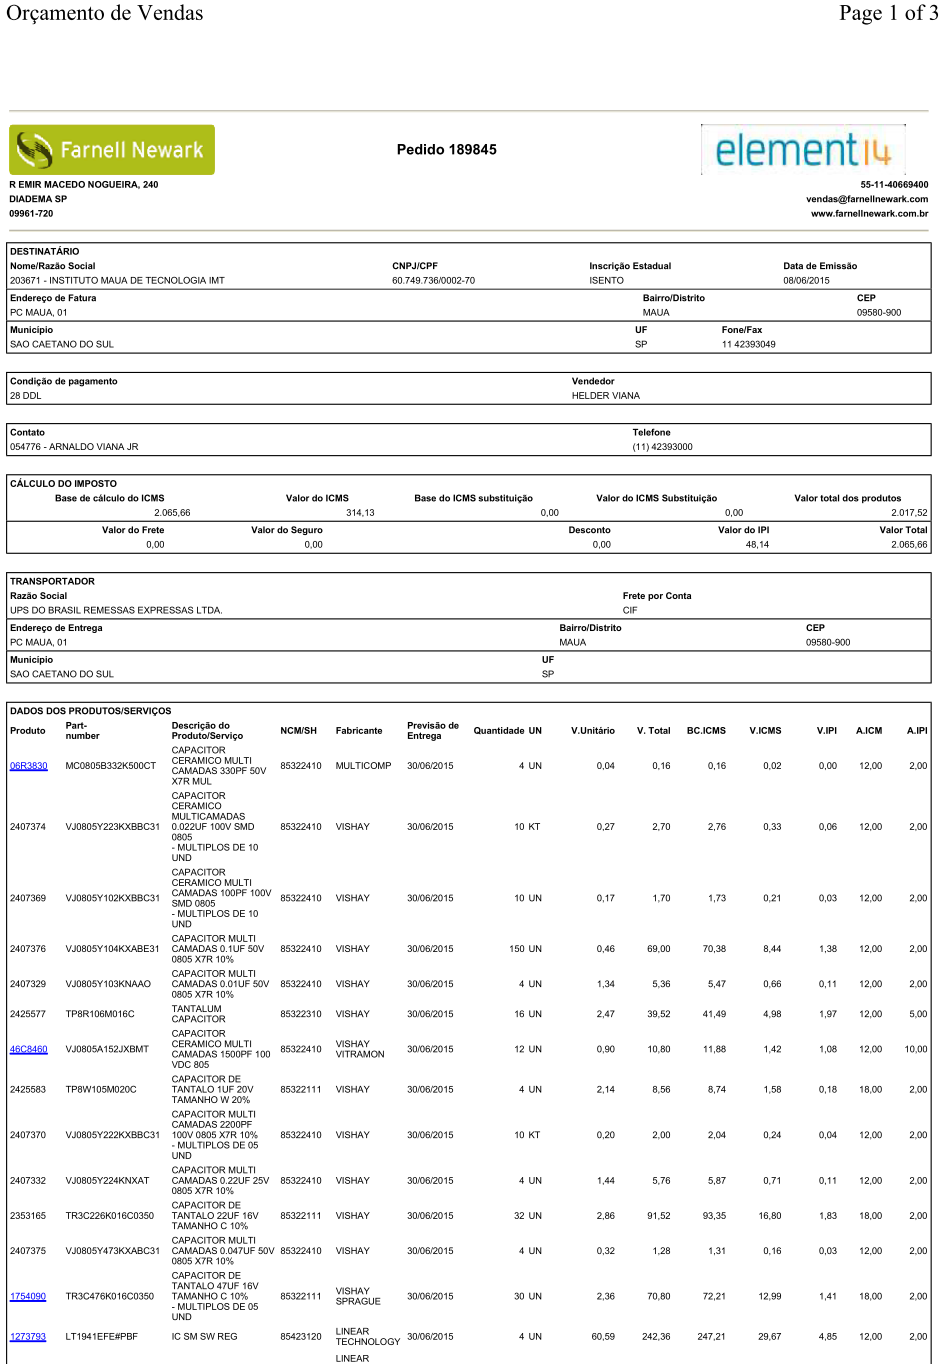
\includegraphics[width=0.85\linewidth]{./anexos/Pedido189845}	
	\end{figure}
	
	\begin{figure}[th]
		\centering
		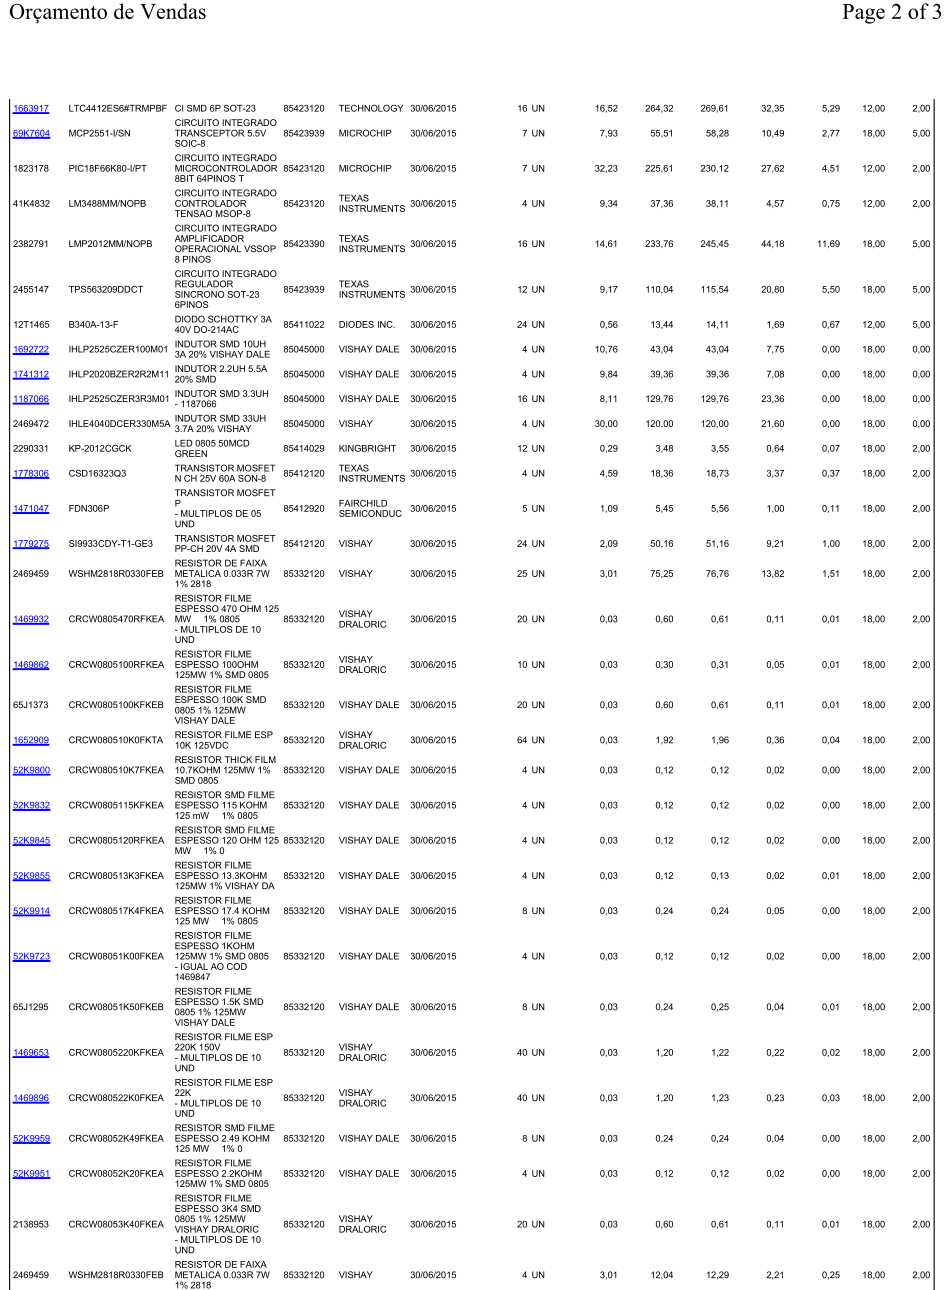
\includegraphics[width=0.9\linewidth]{./anexos/Pedido1898452}	
	\end{figure}
	
	\begin{figure}[th]
		\centering
		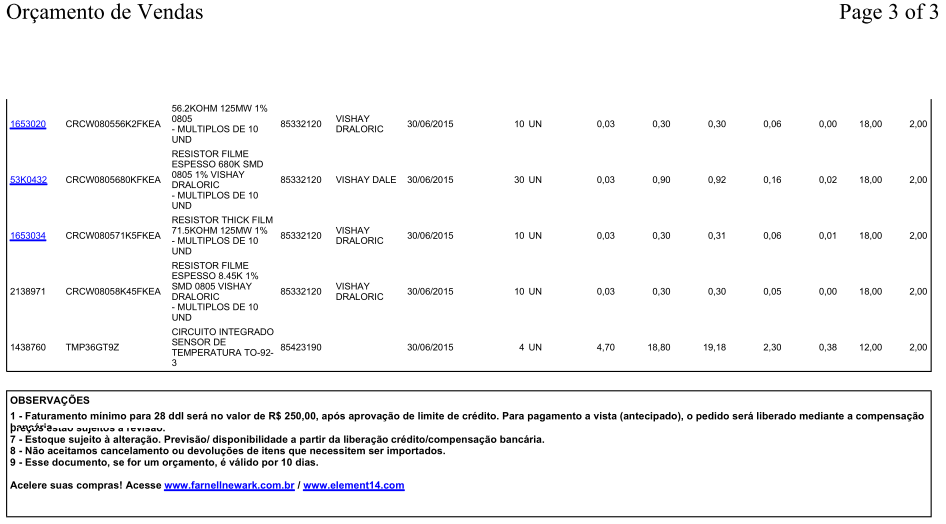
\includegraphics[width=0.9\linewidth]{./anexos/Pedido1898453}	
	\end{figure}
\end{anexosenv}



% ----------------------------------------------------------
% 
% ----------------------------------------------------------
%\chapter[]{}









%---------------------------------------------------------------------
% INDICE REMISSIVO
%---------------------------------------------------------------------
\phantompart
\printindex
%---------------------------------------------------------------------


\end{document}
